% !TeX document-id = {c15effce-b4cb-4262-806c-f65e49a6612b}
% !TeX TXS-program:compile = txs:///pdflatex/[--shell-escape]
\documentclass[mat1]{fmfdelo}
% \documentclass[fin1]{fmfdelo}
% \documentclass[isrm1]{fmfdelo}
% \documentclass[mat2]{fmfdelo}
% \documentclass[fin2]{fmfdelo}
% \documentclass[isrm2]{fmfdelo}

% naslednje ukaze ustrezno napolnite
\avtor{Laura Guzelj Blatnik}

\naslov{Nevronske mreže z vzvratnim razširjanjem napak v funkcijskem programskem jeziku}
\title{Angleški prevod slovenskega naslova dela}

% navedite ime mentorja s polnim nazivom: doc.~dr.~Ime Priimek,
% izr.~prof.~dr.~Ime Priimek, prof.~dr.~Ime Priimek
% uporabite le tisti ukaz/ukaze, ki je/so za vas ustrezni
\mentor{prof.~dr.~Ljupčo Todorovski}
% \mentorica{}
 \somentor{asist.~dr.~Aljaž Osojnik}
% \somentorica{}
% \mentorja{}{}
% \mentorici{}{}

\letnica{2020} % leto diplome

%  V povzetku na kratko opišite vsebinske rezultate dela. Sem ne sodi razlaga organizacije dela --
%  v katerem poglavju/razdelku je kaj, pač pa le opis vsebine.
\povzetek{}

%  Prevod slovenskega povzetka v angleščino.
\abstract{}

% navedite vsaj eno klasifikacijsko oznako --
% dostopne so na www.ams.org/mathscinet/msc/msc2010.html
\klasifikacija{}
\kljucnebesede{} % navedite nekaj ključnih pojmov, ki nastopajo v delu
\keywords{} % angleški prevod ključnih besed

\zapisiMetaPodatke  % poskrbi za metapodatke in veljaven PDF/A-1b standard

% aktivirajte pakete, ki jih potrebujete
% \usepackage{tikz}

% za številske množice uporabite naslednje simbole
\newcommand{\R}{\mathbb R}
\newcommand{\N}{\mathbb N}
\newcommand{\Z}{\mathbb Z}
\newcommand{\C}{\mathbb C}
\newcommand{\Q}{\mathbb Q}

% matematične operatorje deklarirajte kot take, da jih bo Latex pravilno stavil
% \DeclareMathOperator{\conv}{conv}

% vstavite svoje definicije ...
%  \newcommand{}{}


%\usepackage{minted}
\usepackage{neuralnetwork}
\usepackage{epstopdf}
\usepackage{graphicx}
\usepackage{geometry,color}
\usepackage{tikz}
\usetikzlibrary{matrix,chains,positioning,decorations.pathreplacing,arrows}
\usepackage{pgfplots}
\usepackage{pst-plot}
\psset{algebraic=true}

\usepackage{subcaption} 
\usepackage{nicefrac}

%\usepackage[ruled,vlined]{algorithm2e}


\begin{document}
%
\section{Uvod}
%
Človeški možgani so kompleksen organ predvsem zaradi neštetih funkcij, ki jih opravljajo. In zgolj vprašanje časa je bilo, kdaj bodo znanstveniki skoraj neskončne zmožnosti možganov prenesli v računalništvo. Ko so poskušali idejo uresničiti, so si predvsem želeli strukture, ki se bo - podobno kot možgani - sposobna učiti, odzivati na sprememe in prepoznati neznane situacije. Tako je 1949 Donal Hebb v svojem delu prvič predstavil idejo umetnih nevronskih mrežah, kjer se je zgledoval predvsem po možganih. Dvoslojni perceptorn se je rodil nekoliko kasneje, leta 1962 je ta pojem prvi omenil Rosenblatt. Z razvojem storjne opreme se je zanimanje za nevronske mreže zopet povečalo v osemdestih lezih prejšnjega stoletja. Leta 1986 je več razskovalcev neodvisno drug od drugega vpelje teorijo o večslojnih nevronskih mrežah in vzvratnem razširjanju napake. Kljub širokemu spektru uporabe, ki jih nudijo nevronske mreže je interes zanje kasneje nekoliko upadel. V zadnjih letih pa so nevronske mreže zopet vroča tema, predvsem zaradi njihove zmožnosti prepoznavanja slik. Do danes so umetne nevronske mreže močno napredovale, namesto običajnih mrež se vedno bolj uporabljajo globoke nevronske mreže, ki v nekaterih lastnostih celo prekašajo možgane. Kljub vsemu pa so možgani sposobni masrcičesa, česar računalniki ne bodo nikoli.

Diplomska naloga se poglobi v umetne nevronske mreže z vzvratnim razširjanjem napake. Primer take mreže sem tudi implementirala v funkcijskem programskem jeziku OCaml. 
%
\section{Umetne nevronske mreže}
%
%
\subsection{Biološko ozadje}
Kot sugerira že samo ime, se umetne nevronske mreže v marsičem zgledujejo po človeških možganih. Osnovni gradniki možganov so nevroni, ki so med seboj povezani s sinapsami. Prav te goste povezave so ključne za delovanje živčevja. Skozi naše življenje se sinapse spreminjajo po jakosti in številu, ko se učimo se ustvarjajo nove povezave med nevroni, že obstoječe pa postajajo močnejše. Nevron se aktivira le,  ko po sinapsi do njega pride signal s točno določeno frekvenco, ta impulz nato nevron posreduje sosednjim nevronom. Človeške možgane sestavlja $10^{10}$ nevronov, vsak  ima približno $10^4$ sinaps. Umetne nevronske mreže načeloma sestavlja veliko manj nevronov, posledično so zato pri izvajanju operacij veliko hitrejše od možganov. Kot bomo videli v nadaljevanju, je osnovna ideja umetnih nevronskih mrež zelo podobna živčevju v možganih. Lahko bi rekli, da so umetne nevronske mreže zgolj abstraktna poenosatvitev delovanja možganov. 
%
\subsection{Zgradba nevronskih mrež}
Nevronske mreže so sestavljene iz nevronov, ki matematično gledano niso nič drugega kot funkcije. Nevroni so med seboj povezani, vsaka povezava ima svojo težo oziroma utež. Nevrone razdelimo v sloje, pomembno je poudariti, da nevroni v istem sloju med seboj niso povezani, vsak nevron je povezan le z vsemi nevroni v sosednjem (oziroma prejšnjem sloju). Nevronska mreža lahko vsebuje le vhodni in izhodni sloj - takrat govorimo o dvoslojni nevronski mreži. Če se med tema slojema skriva še kakšen skriti sloj, potem mreža postane večslojna. Število nevronov v posameznem sloju tako kot tudi število skritih slojev nevronske mreže je odvisno od problema, ki ga nevronska mreža rešuje.
%
\begin{figure}
\centering
    \begin{neuralnetwork}[height=4]
        \newcommand{\x}[2]{$x_#2$}
        \newcommand{\y}[2]{$y_#2$}
        \newcommand{\hfirst}[2]{\small $h^{(1)}_#2$}
        \newcommand{\hsecond}[2]{\small $h^{(2)}_#2$}
        \inputlayer[count=3, bias=false, title=Vhodni\\sloj, text=\x]
        \hiddenlayer[count=4, bias=false, title=Skriti\\sloj 1, text=\hfirst] \linklayers
        \hiddenlayer[count=3, bias=false, title=Skriti\\sloj 2, text=\hsecond] \linklayers
        \outputlayer[count=2, title=Izhodni\\sloj, text=\y] \linklayers
    \end{neuralnetwork}
\label{mreza}
\caption{Perceptron z dvema skritima slojema nevronov}
\end{figure}
%
Pri mrežah, ki jih bom obravnavala v diplomski nalogi, so vse povezave usmerjene, čeprav je pomembno omeniti, da obstajajo tudi mreže z dvosmernimi povezavami. Usmerjeni nevronski mreži rečemo perceptron, glede na število slojev pa ločimo dvoslojni in večslojni perceptron.  
%
\subsection{Delovanje perceptrona}
Vzemimo dvoslojni perceptron z $m$ nevroni v vhodnem sloju, njihova stanja  označimo z $X_1, X_2, \ldots, X_m$ in $n$ nevroni v izhodnem sloju, označimo jih $Y_1, Y_2, \ldots, Y_{n}$. Običajno sloj nevronov zapišemo v obliki vektorja:
%
\begin{equation*}
X = (X_1, X_2, \dotso, X_m)^\intercal  \quad \text{in} \quad  Y = (Y_1, Y_2, \dotso, Y_n)^\intercal \text{.}
\end{equation*}
%
Uteži med nevroni predstavimo z matriko:
%
\begin{equation*}
M = \begin{bmatrix}
W_{11} &W_{12}  & \cdots & W_{1m}  \\
W_{21}  &W_{22}  &\cdots & W_{2m}  \\
\cdots &  &\cdots &  \\
W_{n1} & W_{n2} & \cdots & W_{nm} 
\end{bmatrix}  
\end{equation*}
%
kjer element matrike $W_{ij}$ predstavlja utež med $i$-tim nevronom v vhodnem sloju in $j$-tim nevronom v izhodnem sloju.
%
\subsubsection{Funkcija kombinacije:}
Stanje $j$-tega nevrona po uporabljeni funkciji aktivacije je sledeče:
%
\begin{equation*}
A_j= \sum_{i}W_{ij}X_i + C_j \text,
\end{equation*}
%
kjer je $W_{ij}$ utež med $i$-tim in $j$-tim nevronom, $C_j$ pa konstanta aktivacije za $j$-ti nevron (njen pomen je pojasnjen v poglavju \ref{bias}). 
Za cel sloj izhodnih nevronov pa lahko funkcijo aktivacije zapišemo z linearno preslikavo:
%
\begin{equation*}
A = WX \text,
\end{equation*}
%
kjer je $W$ matrika uteži, $X$ pa vhodni vektor. Če enačbo zapišemo v vektorski obliki je potrebno upoštevati še konstante aktivacije, zato matriko uteži $W$ in vektor $X$ malo preoblikujemo. Vektorju na konec dodamo še eno komponento z vrednostjo $1$ in dobimo $X =  (X_1, X_2, \dotso, X_m, 1)^\intercal $ matriki uteži pa dodamo še stolpec s konstantami aktivacije za vsak nevron, torej: 
%
\begin{equation*}
M = \begin{bmatrix}
W_{11} &W_{12}  & \cdots & W_{1m}  & C_1\\
W_{21}  &W_{22}  &\cdots & W_{2m}  & C_2\\
\cdots &\cdots  &\cdots &\cdots  &\cdots\\
W_{n1} & W_{n2} & \cdots & W_{nm} & C_n
\end{bmatrix}  
\end{equation*}
%
\subsubsection{Funkcija aktivacije:}
Cilj funkcije aktivacije je normalizirati vrednost, ki jo dobimo s funkcijo kombinacije. Glede na namen uporabe nevronske meže lahko uporabimo različne funkcije aktivacije. Najpogosteje se uporabljaljata stopničasta pragovna funkcija ali pa sigmoidna funkcija.
%
\emph{Stopničasta pragovna funkcija} nevron aktivira le, če je vrodnost dobljena z funkcijo aktivacije nad oziroma pod določeno mejo. Uporaba te funkcije je dokaj omejena. Ker vhodnim podatkom pripiše le dve različni vrednosti, jo lahko uporabimo le pri klasifikaciji v dve kategoriji oziroma za reševanje linearnih problemov. Prav tako jo lahko uporabimo samo pri dvoslojnih perceptronih. Kot bomo videli v nadaljevanju, za večslojne perceptrone ni primerna, saj je njen odvod enak $0$, kar pa pomeni, da za učenje ne moremo uporabiti posplošenega pravila delta.
%
\begin{equation*}
f(x)=
    \begin{cases}
      0, & \text{če } x  \leq 0 \\
      1, & \text{sicer}
    \end{cases} 
\end{equation*}
%
\begin{figure}[!ht]
  \centering
    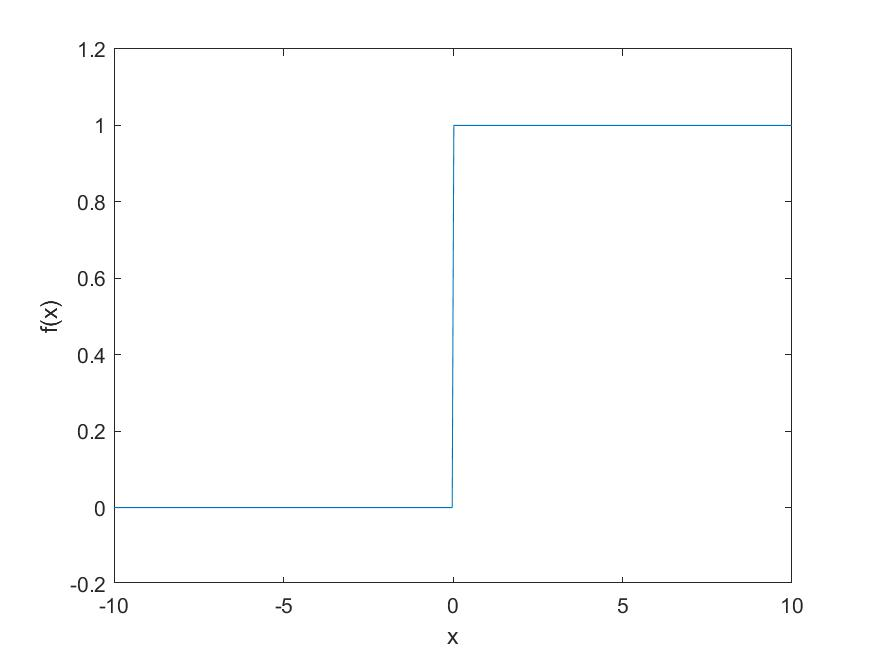
\includegraphics[width=0.5\textwidth]{step_fun.jpg}
  \label{fig:step}
 \caption{Stopničasta pragovna funkcija aktivacije}
\end{figure}
%
\emph{Sigmoidne funkcije} so nelinearne, zato se uporabljajo pri večslojnih perceptornih in reševanju nelinearnih problemov. So zvezne in neskončnokrat zvezno odvedljive, tako jih lahko uporabimo pri posplošenem pravilu delta. Odvisno na kateri interval želimo normalizirati izhodne vrednosti, uporabimo različne sigmoidne funkcije. Primera sigmoidne funkcije sta: 
%
\begin{equation}
f(x) = \frac{1}{1+e^{-x}} \quad in \quad h(x) = \tanh(x) = \frac{e^x-e^{-x}}{e^x+e^{-x}} \text.
\end{equation}
%
Kot lahko vidimo z grafov (slika \ref{fig:sigmoid}) je na intervalu $(-2,2)$ gradient obeh funkcij zelo velik, zato da na omenjenem intervalu mreža pri napovedovanju jasne rezultate in učenje je hitro. Po drugi strani pa je zunaj tega intervala odvod majhen, tako je učenje mreže in posledično napovedovanje zelo počasno in slabo.

Za učenje mreže s posplošenim pravilom delta potrebujemo tudi odvod funkcije aktivacije, ki ga pri zgornjih dveh funkcijah lahko izrazimo z $f(x)$ oziroma $h(x)$ sledeče:
%
\begin{equation}
f'(x) = \frac{e^{-x}}{(1+e^{-x})^2} = f(x)(1-f(x))
\end{equation}
%
\begin{equation}
h'(x) = \left(\frac{\sinh(x)}{\cosh(x)}\right)' = \frac{\cosh^2(x)- \sinh^2(x)}{\cosh^2(x)} = 1 - \tanh^2(x) = 1 - h(x)^2 
\end{equation}
%
\begin{figure}[!th]
\centering
\begin{subfigure}{.5\textwidth}
  \centering
  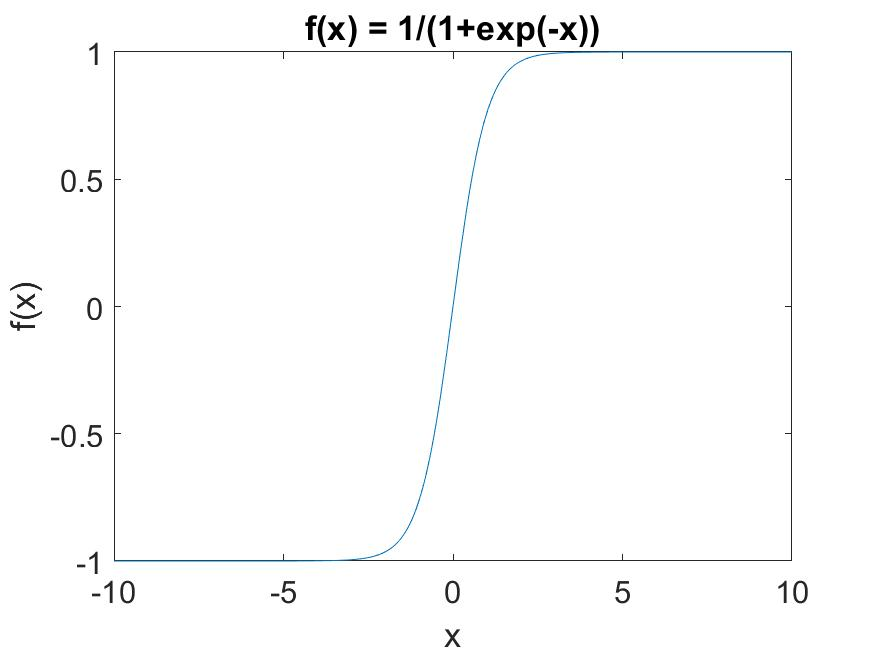
\includegraphics[width=.9\linewidth]{sig_exp.jpg}
\end{subfigure}%
\begin{subfigure}{.5\textwidth}
  \centering
  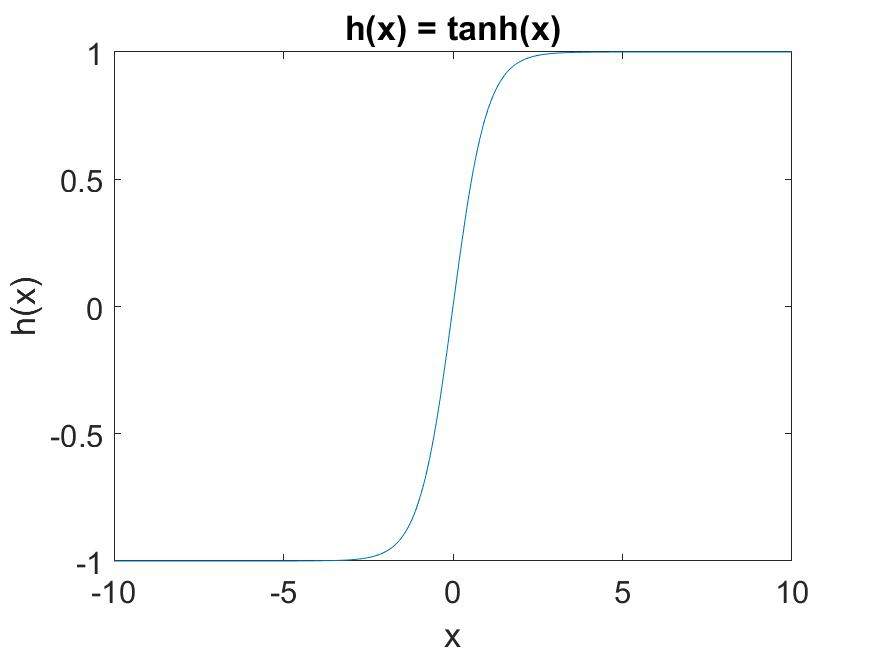
\includegraphics[width=.9\linewidth]{sig_tan.jpg}
\end{subfigure}
\caption{Sigmoidni funkciji aktivacije}
\label{fig:sigmoid}
\end{figure}
%
%

Katero funkcijo aktivacije bomo izbarli je odvisno od problema, ki ga želimo z mrežo obravnavati.
%
\subsubsection{Konstanta aktivacije} \label{bias}
Sloju nevronov pogosto dodamo še en nevron - konstanto aktivacije. To je nevron z vrednostjo $1$, njegova naloga pa je, da funkcijo aktivacije primerno premakne levo oziroma desno po grafu. Brez dodatnega nevrona bi mreža pri vhodnem podatku $X=0$ vedno vračala vrednost $0$, posledično bi bila aproksimacija dane funkcije slaba in rezultati netočni. 

Pomen konstante aktivacije lahko predstavimo tudi s pomočjo linearne funkcije. Vse premice oblike $y = kx$ prečkajo koordinatno izhodišče in tako izgubimo kar nekaj premic. Če pa fuknkciji dodamo še začetno vrednost, ki ustreza pomenu konstante aktivacije, potem lahko z enačno $y= kx + n$ zapišemo poljubno premico. Posledično je mreža bolj fleksibilna, problem bolje aproksimira in vrača bolj točne rezultate. 
%
\subsubsection{Funkcija nevrona}
Izhodni sloj nevronov $Y$ dobimo tako, da vhodni sloj pomnožimo z matriko uteži - temu pravimo funkcija kombinacije, nato pa na tem rezultatu uporabimo še funkcijo aktivacije.\\
%

Če združimo funkcijo kombinacije in funkcijo aktivacije, lahko napišemo pravilo za funkcijo nevrona, tj.~ izračun izhodnih vrednosti nevrona. Za posamezen nevron velja:
%
\begin{equation*}
Y_j = f(\sum_{i}W_{ij}X_i + C_j)
\end{equation*}
%
oziroma v vektorski obliki za cel sloj izhodnih nevronov:
%
\begin{equation*}
Y = f(WX) \text,
\end{equation*}
%
kjer velja, da funkcijo aktivacije uporabimo na vsaki komponenti vektorja $WX$. 
%
\begin{figure}
\centering
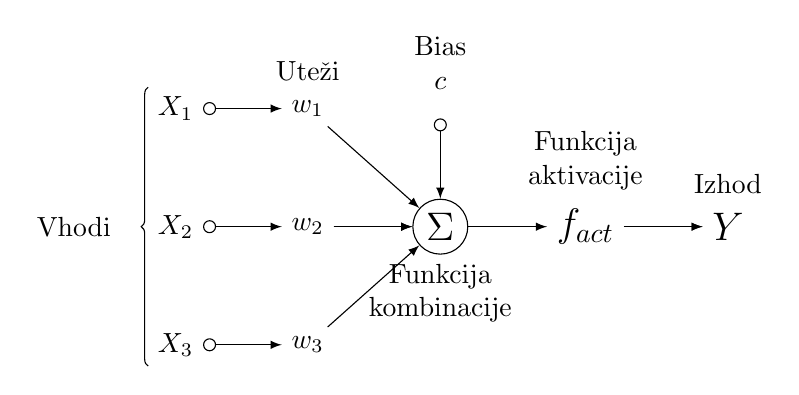
\begin{tikzpicture}[
    % define styles    
    init/.style={ 
         draw, 
         circle, 
         inner sep=2pt,
         font=\Huge,
         join = by -latex
    },
    squa/.style={ 
        font=\Large,
        join = by -latex
    }
]
% Top chain x1 to w1
\begin{scope}[start chain=1]
    \node[on chain=1] at (0,1.5cm)  (x1) {$X_1$};
    \node[on chain=1,label=above:Uteži,join=by o-latex] (w1) {$w_1$};
\end{scope}
% Middle chain x2 to output
\begin{scope}[start chain=2]
    \node[on chain=2] (x2) {$X_2$};
    \node[on chain=2,join=by o-latex] {$w_2$};
%\node[on chain=2,squa,label=above:{\parbox{6cm}{\centering Funkcija\\ kombinacije}}]{$\displaystyle\Sigma$};

    \node[on chain=2,init, squa,label=below:{\parbox{4cm}{\centering Funkcija\\ kombinacije}}] (sigma) {$\displaystyle\Sigma$};
    \node[on chain=2,squa,label=above:{\parbox{2cm}{\centering Funkcija\\ aktivacije}}]   {$f_{act}$};
    \node[on chain=2,squa,label=above:Izhod,join=by -latex] {$Y$};
\end{scope}
% Bottom chain x3 to w3
\begin{scope}[start chain=3]
    \node[on chain=3] at (0,-1.5cm) 
    (x3) {$X_3$};
    \node[on chain=3,join=by o-latex]
    (w3) {$w_3$};
\end{scope}
% Bias
\node[label=above:\parbox{2cm}{\centering Bias \\ $c$}] at (sigma|-w1) (b) {};

% Arrows joining w1, w3 and b to sigma
\draw[-latex] (w1) -- (sigma);
\draw[-latex] (w3) -- (sigma);
\draw[o-latex] (b) -- (sigma);
% left hand side brace
\draw[decorate,decoration={brace,mirror}] (x1.north west) -- node[left=10pt] {Vhodi} (x3.south west);
\end{tikzpicture}
\caption{Funkcija nevrona}
\label{Funkcija nevrona}
\end{figure}
%
\subsection{Lastnosti nevronskih mrež}
Nevronske mreže odlikuje kar nekaj pozitivnih lastnosti. Najpomembnejše med njimi so sledeče:

\textbf{Paralelizabilnost: }Posamičen nevron deluje relativno neodvisno od ostalih nevronov. Paralelizabilnost posledično pomeni zelo hitre operacije in omogoča uporabo nevronskih mrež pri reševanju kompleksnih problemov.

\textbf{Stabilnost: }Izgubljen ali nedelujoč nevron le malo pokvari natančnost delovanja nevronske mreže (več kot je takih nevronov, manj natančna je nevronska mreža). Nevronske mreže so tako stabilne v smislu uničenih nevronov in njihovih povezav. Poleg tega pa so stabilne tudi v smislu nepopolnih podatkov. To pomeni, da mrežo lahko naučimo pravilnega delovanja, tudi če v učnih priemrih del podatkov manjka. Velja pa, da bolj nepopolni kot so podatki, slabša je aproksimacija nevronske mreže.

\textbf{Matematično ozadje: }Cilj nevronske mreže je aproksimirati poljubno funkcijo in kasneje na podlagi te aproksimacije napovedati vrednosti pri poljubnih vhodnih podatkih. Pri računanju se nevronske mreže močno opirajo na linearno algebro, linearnime preslikave, lastne vrednosti in vektorje ter negibne točke.

Glavna pomanjkljivost nevronskih mrež je določanje topologije mreže. Medtem ko je število nevronov v vhodnem in izhodnem sloju določeno s problemom, je število nevronov v posameznem skritem sloju in število skritih slojev odvisno od posameznega primera. Idealno topologijo nevronske mreže je tako težko doseči, do nje lahko pridemo le s empirično s poskušanjem. Še ena slaba lastnost pa je nezmožnost razlaganja odločitev (ang.~ balckbox). Zaradi kompleksne strukture je vsak rezultat mreže produkt večih neodvisnih operacij nevronov, ki jih ne moremo razložiti.

%
%
\subsection{Uporaba nevronskih mrež}
Z razvojem strojne opreme v zadnjih letih so močno napredovale tudi nevronske mreže. Razvite tudi hitrjše implementacije algoritmov, posledično je zaradi njihove efektivnosti uporaba nevronskih mrež danes zelo pogosta v industriji. Ko nevronsko mrežo z učnimi primeri naučimo pravilnega delovanja, se mreža zna odzvati na nepoznane situacije. Tako lahko, zaradi njihove splošnosti in sposobnosti sprejetja velikega števila vhodnih podatkov, nevronske mreže uporabimo za reševanje najrazličnejših probleme. Zato se dandanes uporabljajo na skoraj vseh mogočih področjih. Dva najpomembenjša namena uporabe sta napovedovanje in klasifikacija. Primeri uporabe v industriji so: 
\begin{itemize}
\item prepoznavanje in klasifikacija slik: konkretno podjetje Google uporablja nevronske mreže za prepoznavanje slik, ki jih nato opremi s ključnimi besedami,
\item prepoznavanje ročno napisanih besedil,
\item prepoznavanje  govora, tu bi veljalo izpostaviti podjete Miscrosoft, ki je razvilo nevronsko mrežo, ki govorjeno angleščino prevaja v kitajščino,
\item kontrola kvalitete v produkciji,
\item v zdravstvu se uporabljajo za določanje pacientove diagnoze,
\item napovedovanje različnih vrednosti glede na trenutne trende.
\end{itemize}
%
\section{Učenje}
Najprej je smiselno definirati, kaj pojem učenje sploh pomeni. Po \cite[str.~37]{kononenko} za učenje potrebujemo sistem, ki strmi k izpolnitvi določene naloge oziroma cilja. Pred učenjem sistem ni sposoben zadostno opraviti naloge. S ponavljanjem določenih opravil poskušamo sistem pripraviti do tega, da bo deloval bolje, kjer je bolje lahko hitreje, ceneje, bolj pravilno\ldots Učenje lahko torej definiramo kot zaporedje ponovitev, kjer pri vsaki ponovitvi skušamo zmanjšati napako tako, da bi se zastavljenemu cilju čimbolj približali. 

Obstaja kar nekaj različnih pravil, kako umetno nevronsko mrežo naučiti pravilnega delovanja. V svoji diplomski nalogi sem se osredotočila na posplošeno pravilo delta oziroma vzvratno razširjanje napake, ki je nekako standaren algoritem za učenje pri večslojnih perceptronih. 
%
\subsection{Nadzorovano učenje}
Vzvratno razširjanje napake je primer nadzorovanega učenja. Za tako učenje potrebujemo učne primere - torej vhodne podatke in vredosti, ki želimo, da jih mreža pri danih vhodnih podatkih vrača. Cilj učenja je najti funkcijo, ki bo najbolje aproksimirala relacijo med vhodnimi in izhodnimi podatki. Pri vzvratnem razširjanju napake do take funkcije pridemo tako, da spreminjamo vrednosti na utežeh, pri čemer poskušamo minimalizirati napako med želenim in dobljenim izhodom mreže.

Potrebno je omeniti še, da poleg nadzorovanega učenja poznamo tudi nenazdrovano učenje. Tu izhodnih podatkov nimamo. Mreža vhodne podatke obdela po svojih kriterijih in poskuša najti strukturo, ki povezuje vhodne podatke med seboj. Nenazdorovano učenje se praviloma ne uporablja pri nevronskih mrežah.
\subsection{Pravilo delta}
Pravilo delta je eno izmed pravil, ki ga lahko uporabimo pri učenju nevronske mreže, ponavadi se uporablja na dvoslojnih perceptronih.Če je mreža večslojna, potem govorimo o vzvratnem razširjanju napake oziroma posplošenem pravilu delta. Za pravilom delta stoji povsem preprosta ideja. Najprej uteži med nevroni poljubno nastavimo(pomembno je le, da niso vse uteži nastavljene na 0), nato na izbranem testnem primeru izračunamo za koliko se je naša mreža zmotila glede na pričakovan izhod. Tako dobimo napako s pomočjo katere lahko vrednosti na utežeh popravimo tako, da minimaliziramo dobljeno napako. Postopek ponavljamo na ostalih učnih primerih, dokler se uteži ne ustalijo (včasih lahko isti učni primer uporabimo tudi večkrat). Takrat se učenje konča.

Za začetek vzemimo preprost dvoslojni perceptron z enim izhodnim nevronom $Y$, število vhodnih nevronov je poljubno. Pravilo delta pri spreminjanju vrednosti uteži upošteva razliko med želenim in dobljenim izhodom mreže. Tako definiramo napako mreže kot kvadrat razlike omenjenih izhodov:
%
\begin{equation}
\begin{aligned}
E(l) &= (d(l)-Y(l))^2 \\
&= (d(l)-WX(l))^2
\end{aligned}
\end{equation}
%
kjer je $d(l)$ želen izhod in $Y(l)= WX(l)$ z mrežo izračunana vrednost pri $l$-tem učnem primeru, vhodnem vektorju $X(l)$ in matriki uteži $W$.

Pravilo delta temelji na gradientnem iskanju, vektor uteži popravljamo v negativni smeri odvoda napake po utežeh. Izračunamo še odvod napake po utežeh:
%
\begin{equation*}
\frac{dE(l)}{dW}= -2(d(l)-WX(l))X(l)
\end{equation*}
%
Sedaj lahko zapišemo enačbo za pravilo delta in nove vrednosti uteži $W^{N}$:
%
\begin{equation}
\begin{aligned}
W^{N} &= W - \eta\frac{dE(l)}{dW} \\
&= W + \eta(d(l)-WX(l))X(l)
\label{utezi}
\end{aligned}
\end{equation}
%
V zgornji enačbi $\eta$ predstavlja hitrost učenja in določa kako hitro bodo uteži konvergirale k optimalnim. 

\subsubsection{Gradientno iskanje} 
Za pravilom delta stoji gradientno iskanje. To je v bistvu iskanje lokalnega minimuma. Začnemo na naključni točki na grafu (zato utežem na začetku nastavimo naključne vrednosti) in se nato v vsakem koraku premaknemo po krivulji v smeri negativnega odvoda, to je smer, kjer funkcija najhitreje pada. Dolžino vsakega premika pri učenju nevronskih mrež določa stopnja učenja $\eta$, zato je pomembno kakšno vrednost zanjo izberemo.

\subsection{Vzvratno razširjanje napake}
%IDEJA in opis
Vzvratno razširjanje napake temelji na pravilu delta. Problem se pojavi, ker uteži med skritimi sloji niso direktno odvisne od napake med izhodnim stanjem in želeno vrednostjo, zato moramo pravilo malo prilagoditi. Ko popravljamo uteži, to počnemo od izhodnega sloja nevronov proti vhodnemu (od tod tudi ime -  vzvratno razširjanje napake oziroma \emph{backpropragation} v anglrščini). 

\subsubsection{Notacija}
Definirajmo notacijo, ki jo bomo uporabili pri izpeljavi vzvratnega razširjavnja napake. 
\begin{itemize}
\item $X_{i}$ označuje $i$-ti nevron v vhodnem sloju.
\item $H_{ki}$ označuje $i$-ti nevron v $k$-ti skriti plasti.
\item $Y_i$ označuje $i$-ti nevron v izhodni plasti
\item $W^{(k)}_{ij}$ označuje utež med $i$-tim nevronom v  $k-1$ plasti in $j$-tim nevronom v $k$-ti plasti
\item $A_{ki}$ označuje stanje $i$-tega nevrona v $k$-ti skriti plasti po uporabljeni funkciji kombinacije: $A_{kj} = \sum^{N_{k-1}}_{j=1}W^{(k)}_{ij}X_j$, poseben primer je stanje $i$-tega nevrona v izhodni plasti, ki ga označimo z $A_i$
\end{itemize}

\subsubsection{Izpeljava vzvratnega razširjanja napake}
Vzemimo splošen večsojen perceptron z $N_X$ nevroni v vhodnem sloju in $N_Y$ nevroni v izhodnem sloju. Nevronska mreža naj sestoji iz $m$ skritih slojev, $m>0$, vsak skriti sloj pa naj vsabuje $N_k$ nevronov, kjer velja $1\leq k \leq m$. 

Preden se lotimo popravljanja uteži, moramo za dani $l$-ti učni primer izračunamo izhodne vrednosti. To storimo tako, da na vsakem nevronu uporabimo funkcijo aktivacije in kobinacije. Za $i$-ti nevron v prvem skritem sloju lahko zapišemo:
%
\begin{equation*}
H_{1i}(l) = f\left( \sum^{N_X}_{j=1}{W^{(1)}_{ij}X_j(l)}\right)
\end{equation*}
%
in
%
\begin{equation*}
A{1i}(l) =\sum^{N_X}_{j=1}{W^{(1)}_{ij}X_j(l)}
\end{equation*}
%
Za poljubni $k$-ti sktiti sloj, kjer je $1\leq k \leq m$ ,tako zapišemo:
%
\begin{equation*}
H_{ki}(l) = f(A_{ki}(l))\text,
\end{equation*}
%
kjer je
%
\begin{equation*}
A_{ki}(l) = \sum^{N_{k-1}}_{j=1}W^{(k)}_{ij}H_{k-1,j}(l)\text.
\end{equation*}
%
V zgornji enačbi $H_{k-1,j}$ označuje že izračunane vrednosti nevronov v predhodnem sloju.
 
 V izhodnem sloju dobimo vrednosti, ki nas najbolj zanimajo. Velja:
%
\begin{equation*}
Y_{i}(l) = f(A_{i}(l)) \quad \text{in} \quad A_{i}(l) = \sum^{N_{m}}_{j=1}{W^{(m+1)}_{ij}H_{m,j}(l)}\text.
\end{equation*}
%
Tako smo dobili izhodne vrednosti, ki jih je izračunala naša mreža. Vrednosti primerjamo s tistimi, ki bi si jih želeli dobiti za dani $l$-ti učni primer. Za posamezen nevron ozančimo sledeče:
%
\begin{equation}
e_i(l) = d_i(l) - Y_i(l)\text,
\end{equation}
lahko pa enačbo zapišemo tudi v vektoski obliki:
\begin{equation*}
e(l) = d(l) - Y(l)\text.
\end{equation*}
Podobno kot pri pravilu delta, napaki celotne nevronske mreže za $l$-ti učni primer definiramo:
%
\begin{equation}
E(l) = \frac{1}{2}\sum^{N_Y}_{i=1}e_i^2(l)
\label{napaka}
\end{equation}
%
Napako želimo minimalizirati in podobno kor prej s pomočjo gradientnega iskanja uteži popraviti v smeri negativnega odvoda napake $E$. Nove uteži izračunamo s pomočjo enake formule kot prej (enačba \eqref{utezi}):
\begin{equation*}
W^{N} = W - \eta \frac{dE}{dW}, 
\end{equation*}
%
kjer $\eta$ označuje stopnjo učenja. 

Pri izračunu zgornjega odvoda si bomo pomagali s verižnim pravilom za odvajanje. Za izhodni sloj je napako enostavo izračunati. Problem se pojavi pri skritih slojih, saj uteži niso direktno odvisne od napake. Kot bomo videli v nadaljevanju, si bomo tudi v tem primeru pomgali z verižnim pravilom. 

Najprej razpišimo formulo \eqref{napaka}, kjer upoštevamo formuli za $e_i$ in $Y_i$:
\begin{equation*}
\begin{aligned}
E(l) &= \frac{1}{2}\sum^{N_Y}_{i=1}e_i^2(l) \\
&=\frac{1}{2}\sum^{N_Y}_{i=1}{(d_i(l) - Y_i(l))}^2(l) \\
&= \frac{1}{2}\sum^{N_Y}_{i=1}{(d_i(l)-f(\sum^{N_m}_{j=1}{W^{(m+1)}_{ij}H_{m,j}(l)))}}^2(l)  
\end{aligned}
\end{equation*}
%
 Sedaj za izračun odvoda uporabimo verižno pravilo,  formulo razpišemo na posamezno utež:
%
\begin{equation}
\frac{\partial E(l)}{\partial W^{(m+1)}_{ij}} = \frac{\partial E(l)}{\partial e_i(l)}
\frac{\partial e_i(l)}{\partial Y_i(l)} 
\frac{\partial Y_i(l)}{\partial A_i(l)}
\frac{\partial A_i(l)}{\partial W^{(m+1)}_{ij}}
\end{equation}
%
Zgornje parcialne odvode pa lahko ob pomoči definicij posameznih izrazov zapišemo sledeče:
%
\begin{equation}
\frac{\partial E(l)}{\partial e_i(l)} = \frac{\partial (\frac{1}{2}\sum^{N_Y}_{i=1}e_i^2(l))}{\partial e_i(l)}=e_i(l)
\end{equation}
%
\begin{equation}
\frac{\partial e_i(l)}{\partial Y_i(l)}= \frac{\partial (d_i(l) - Y_i(l))}{\partial Y_i(l)} = -1
\end{equation}
%
\begin{equation}
\frac{\partial Y_i(l)}{\partial A_i(l)} = \frac{\partial (f(A_i(l))) }{\partial A_i(l)} =f'(A_i(l))
\end{equation}
%
\begin{equation}
\frac{\partial A_i(l)}{\partial W^{(m+1)}_{ij}} =\frac{\partial \sum^{N_m}_{j=1}W_{ij}^{(m+1)}H_{m,j}(l)}{\partial W^{(m+1)}_{ij}} = H_{mj}(l)
\end{equation}
%
Pri tem velja, da je $f'$ odvod funkcije aktivacije in je odvisen od tega, katero funkcijo aktivacije uporabimo. 

Zaradi boljše preglednosti parcialni odvod zapišemo še malo drugače:
\begin{equation*}
\begin{aligned}
\frac{\partial E(l)}{\partial W^{(m+1)}_{ij}} = \frac{\partial E(l)}{\partial A_i(l)}\frac{\partial A_i(l)}{\partial W^{(m+1)}_{ij}} 
\end{aligned}
\end{equation*}
%
Če upoštevamo zgoraj izračunani odvod dobimo: 
%
\begin{equation*}
\frac{\partial E(l)}{\partial W^{(m+1)}_{ij}} = \frac{\partial E(l)}{\partial A_i(l)}H_{mj}(l) 
\end{equation*}
%
Označimo: 
%
\begin{equation}
\frac{\partial E(l)}{\partial A_i(l)} = \Delta^{(m+1)}_i(l)
\label{eq:deltaY}
\end{equation}
%
Združimo vse zgornje rezultate in zapišemo pravilo za izračun novih uteži pri izhodnem sloju:
%
\begin{equation}
\begin{aligned}
W^{N(m+1)}_{ij} &= W ^{(m+1)}_{ij}- \eta \frac{dE(l)}{dW_{ij}^{(m+1)}} \\
&= W ^{(m+1)}_{ij} -\eta  \Delta^{(m+1)}_i (l)H_{mj}(l)\\
&= W ^{(m+1)}_{ij} -\eta e_i(l) f'(A_i(l))H_{mj}(l)\\
\end{aligned}
\end{equation}
%
Tako smo izpeljali pravilo za spremembno uteži, ki povezujejo izhodni sloj s predhodnikom. 

Vzvratno razširjanje napake pride do izraza šele pri skritih slohjih. Ker ne moremo direktno izračunati napake $e_i$, si pri računanju pomagamo z že spremenjenimi utežmi v izhodnem sloju in pa $\Delta^{(m+1)}$, ki smo ga spotoma izračunali. Za uteži, ki povezujejo predzadnji in zadnji skriti sloj lahko ob upoštevanju verižnega pravila zapišemo:
%
\begin{equation*}
 \frac{\partial E(l)}{\partial W^{(m)}_{ij}} = \frac{\partial E(l)}{\partial A_{mi}(l)} \frac{\partial A_{mi}(l)}{\partial W^{(m)}_{ij}}
%= \Delta^{(m)}_i (l)H_{m-1,j}
\end{equation*}
%
%
%OD TU NAPREJ DELAJ
Drugi člen odvoda enostavno izračunamo
\begin{equation*}
\frac{\partial A_{mi}(l)}{\partial W^{(m)}_{ij}} = H_{m-1,j}(l)
\end{equation*}
%
in podobno kot prej označimo
%
\begin{equation*}
\frac{\partial E(l)}{\partial A_{mi}(l)} = \Delta^{(m)}_i(l)
\end{equation*}

Zopet uporabimo verižno pravilo za odvajanje in zapišemo:
%
\begin{equation*}
\Delta^{(m)}_i(l) = \frac{\partial E(l)}{\partial A_{mi}(l)}  = \frac{\partial E(l)}{\partial H_{mi}(l)}\frac{\partial H_{mi}(l)}{\partial A_{mi}(l)}
\end{equation*}
%
Odvod $\nicefrac{\partial H_{mi}(l)}{\partial A_{mi}(l)}$ je odvod funkcije aktivacije:
%
\begin{equation*}
\frac{\partial H_{mi}(l)}{\partial A_{mi}(l)} =  f'(A_{mi}(l)) \text,
\end{equation*}
%
$\nicefrac{\partial E(l)}{\partial H_{mi}(l)}$ pa zopet razpišemo s pomočjo verižnega pravila
%
\begin{equation*}
\begin{aligned}
\frac{\partial E(l)}{\partial H_{mi}(l)} &=  \sum^{N_Y}_{j=1} \frac{\partial E(l)}{\partial A_j(l)}\frac{\partial A_j(l)}{\partial H_{mi}(l)}  \\
& =   \sum^{N_Y}_{j=1} \frac{\partial E(l)}{\partial A_j(l)}\frac{\partial(\sum^{N_m}_{p=1} W^{N (m+1)}_{pj}H_{mp}(l))}{\partial H_{mi}(l)} \\
&= \sum^{N_Y}_{j=1} \frac{\partial E(l)}{\partial A_j(l)} W^{N (m+1)}_{ji}
\end{aligned}
\end{equation*}
%
Pri tem velja, da so elementi matrike uteži $W^{N(m+1)}$ vrednosti, ki smo jih že popravili v prejšnjem koraku. Uporabimo enačbo \eqref{eq:deltaY} in izrazimo vrednost $\Delta^{(m)}_i(l)$ sledeče:
%
\begin{equation*}
\begin{aligned}
\Delta^{(m)}_i(l) &= f'(A_{mi}(l))  \sum^{N_Y}_{j=1} \frac{\partial E(l)}{\partial A_j(l)} W^{N (m+1)}_{ji} \\
&= f'(A_{mi}(l))  \sum^{N_Y}_{j=1} \Delta ^{(m+1)}_j(l)W^{N (m+1)}_{ji}
\end{aligned}
\end{equation*}
%
Vse združimo in vstavimo v enačbo za izračun spremenjenih uteži $W^{N(m)}$ ter dobimo:
%
\begin{equation}
\begin{aligned}
W^{N(m)}_{ij} &= W^{(m)}_{ij} - \eta\frac{dE(l)}{dW_{ij}^{(m)}} \\
&= W ^{(m)}_{ij} -\eta  \Delta^{(m)}_i (l)H_{m-1,j}(l)\\
&= W ^{(m)}_{ij} -\eta f'(A_{mi}(l))  \left(\sum^{N_Y}_{p=1} \Delta ^{(m+1)}_p(l)W^{N (m+1)}_{pi}\right)H_{m-1,j}(l)\\
\end{aligned}
\end{equation}
%
Za uteži $W^{(k)}$, ki povezujejo poljuben $k-1$ in $k$-ti skriti sloj, kjer je $1 < k < m$, podobno zapišemo:
%
\begin{equation*}
\frac{\partial A_{ki}(l)}{\partial W^{(k)}_{ij}} = H_{k-1,j}(l)
\end{equation*}
%
in 
%
\begin{equation*}
\Delta^{(k)}_i(l) =  f'(A_{ki}(l))  \sum^{N_{k+1}}_{j=1} \Delta ^{(k+1)}_j(l)W^{N (k+1)}_{ji}
\end{equation*}
%
Spremenjene uteži nato izračunamo sledeče:
%
\begin{equation}
\begin{aligned}
W^{N(k)}_{ij}&= W ^{(k)}_{ij} -\eta  \Delta^{(k)}_i (l)H_{k-1,j}(l)\\
&= W ^{(k)}_{ij} -\eta f'(A_{ki}(l))  \left(\sum^{N_{k+1}}_{p=1} \Delta ^{(k+1)}_p(l)W^{N (k+1)}_{pi}\right)H_{k-1,j}(l)\\
\end{aligned}
\end{equation}
%
Ostane nam le še matrika uteži $W^{(1)}$, ki povezuje vhodni sloj s prvim skritim slojem. Zapišemo:
%
\begin{equation*}
\frac{\partial A_{1i}(l)}{\partial W^{(1)}_{ij}} = X_j(l)
\end{equation*}
%
in 
%
\begin{equation*}
\Delta^{(1)}_i(l) =  f'(A_{1i}(l))  \sum^{N_{2}}_{j=1} \Delta ^{(2)}_j(l)W^{N (2)}_{ji}
\end{equation*}
%
Uteži pa popravimo po sledečo formuli:
%
\begin{equation}
\begin{aligned}
W^{N(1)}_{ij}&= W ^{(1)}_{ij} -\eta  \Delta^{(1)}_i (l)X_j(l)\\
&= W ^{(1)}_{ij} -\eta f'(A_{1i}(l))  \left(\sum^{N_{2}}_{p=1} \Delta ^{(2)}_p(l)W^{N (2)}_{pi}\right)X_j(l)\\
\end{aligned}
\end{equation}
%
%
Tako smo izpeljali pravilo za računanje spremembe uteži pri vzvratnem razširjanju napake.
%
\subsection{Lastnosti vzvratnega razširjanja napake}
Kljub temu, da je vzvratno razširjanje napake zelo priljubljeno pravilo pri učenju nevronskih mrež, ima tudi nekaj pomanjkljivosti. 

Gradientno iskanje temelji na iskanju lokalnega minimuma, posledično uteži ne konvergirajo vedno k globalno najboljši izbiri. Lahko se zgodi, da bo matrika uteži konvergirala k lokalnemu optimumu, taka mreža ne bo dajala zadovoljivih rezultatov. Kam bodo uteži konvergirale je odvisno predvsem od njihove začetne izbire. Če med učenjem pride do omenjenega problema moramo izbrati novo naključno matriko uteži in učenje ponoviti v upanju, da bodo uteži tokrat konvergirale k optimalnim.

Naslednji problem, ki se pojavi kot posledica gradientnega iskanja je določanje parametra $\eta$. Stopnja učenja določa kako hitro in kam bo mreža konvergirala. Žal pa ni pravila, ki bi določal kakšno vrednost je za $\eta$ najbolje izbrati. Do take vrednosti lahko pridemo le s poskušanjem.

Slabost vzvratnega razširjanja napake je tudi to, da je za učenje nevronske mreže potrebno zelo veliko število učnih primerov. Ponavadi se to število giblje med nekaj $10000$ in $100000$. Posledično je učenje lahko zelo zamudno.

Potrebno je omeniti še časovno zahtevnost, zaradi svoje kompleksne zgradbe so nevronske mreže zelo časovno potratne in njihovo učenje praviloma ni hitro. Z večjo mrežo le to zahtevnost še povečamo. Kljub temu, pa lahko z različnimi implementacijami malo vplivamo na hitrost mreže.
%
\subsection{Napaka in varianca}
Po končanem učenju lahko preverimo napako in varianco nevronske mreže. Ta podatka povesta, kako uspešni smo bili pri aproksimaciji funkcije. Ker gre za aproksimacijo, bo napaka vedno prisotna, želimo pa, da bi bila le ta čim manjša. Omenjeni količini izračunamo na poljubnem testnem primeru.

S $t$ označimo točno vrednost, ki bi jo želeli dobiti, s $\hat{t}$ pa vrednost, ki jo mreža vrne. Z $E[\hat{t}]$ označimo pričakovano napoved, to je povprečje vrednosti, ki jih dobimo, če mrežo poženemo na  več testnih primerih. Napako mreže pri $t$-tem učnem primeru označimo z $N(t)$ in izračunamo sledeče:
%
\begin{equation}
N(t) = E[\hat{t}] - t
\end{equation}
%
Ptoblem se pojavi, če točne vrednosti $t$ ne poznamo. Včasih lahko iz ostalih podatkov sklepamo kakšna bi ta vrednost morala biti ali pa jo poskusimo oceniti na kakšen drugačen način. Nadalje definiramo še varianco $Var(t)$, ki meri občutljivost mreže na dan učni nabor podatkov:
%
\begin{equation}
Var(\hat{t}) = E[E[\hat{t}] -\hat{t}]^2
\end{equation}
%
\begin{equation}
\begin{aligned}
E[(\hat{t}-t)^2] &= E[(\hat{t} -E[\hat{t}] + E[\hat{t}] - t)^2]  \\
&= (E[\hat{t}] - t)^2 +E[E[\hat{t}] -\hat{t}]^2\\
&= N(t)^2 + Var(\hat{t})
\end{aligned}
\end{equation}
%
Včasih se lahko zgodi, da napaka med učenjem začne rasti. Pomembno je, da učenje takrat prekinemo, saj lahko sicer pride do preprileganja (ang. overfitting). Preprileganje pomeni, da mreža zelo dobro deluje na učnih primerih (napaka je tu majhna), aproksimacija za poljuben primer pa ni natančna. 

V nasprotju z preprileganjem p
%
%-stopnjo učenja moramo določiti empirično, stopnja učenja vpliva na gradientno metodo, eta vpliva kako hitro bomo prišli do minimuma 
%-topologijo določimo empirično, ni pravila, s poskušanjem
%-ni nujno da konvergira k optimalni mreži, lahko limitira k lokalnemu optimumu kar ni generalno najbolje, kam bo limitiralo odvisno oz začetnih uteži, če ni ok učenje ponovimo
%- potrebno veliko število učnih primerov da mreža pravilno deluje, 10 alo 100 tisoč da dejansko ok deluje
%
%Rešitev: 
%
\subsection{Normalizacija podatkov}
Vhodne in izhodne podatke je pred učenjem potrebno normalizirati. Obstaja več pravil za normalizacijo, najbolj pogosta sta min-max normalizacija in z-score normalizacija.
%
\subsubsection{Min-max normalizacija}

%
\subsection{Z-score normalizacija}
%
\section{Funkcijski programski jezik OCaml}
OCaml spada med funkcijske programse jezike. Poleg funkcijskih poznamo še objektne in proceduralne programske jezike. Vsi načini programiranja imajo svoje prednosti in slabosti. Ponavadi se za programski jezik odločimo glede problem, ki ga želimo rešiti. 

Sama sem se za OCaml odločila, ker so implementacije nevronskih mrež v funkcijskih programskih jezikih zelo redke in mi je to predstavljalo izziv. 
%
\subsubsection{Lastnosti funkcijskih programskih jezikov}
V funkcijskem programiranju so osnovni objekti funkcije. To pomeni, da lahko funkcije sprejmejo ozrioma vračajo druge funkcije, poleg tega lahko funkcije shranimo v podatkovne strukture. Funkcijam, ki kot argument sprejmejo funkcije pravimo \emph{funkcije višjega reda}. Ena izmed osnovnih funkcij višjega reda je na primer funkcija map. Le ta sprejme podatkovno strukturo, naprimer seznam ali tabelo, in na vsakem njenem elementu uporabi funkcijo, ki smo jo podali kot argument.

%\begin{minted}{ocaml}
%type 'a t = { name : string; mutable info : 'a};;
%let p = { name = "John"; info = 23 };;
%let double_quote = '"'
%let broken_highlight = ()
%\caption{Example from external file}
%\label{listing:3}
%\end{minted}

% To pomeni, da lahko kot spremenljivko funkciji podamo kar funkcijo. Tako funkcijam, ki kot argument lahko sprejmejo drugo funkcijo, pravimo funkcije višjega reda (higher-order function). Funkcijsko programiranje je zelo efektivno pri rekurzivnih funkcijah. 

%Primer z mapom??

\subsection{Lastnosti OCamla}

- je hiter
- kodo lahko pišemo tudi proceduralno ali objektno, ni strikten funkcijskinjezik
-tipi
- varen (ni napak)
- nespremenljivi tipi, to ni vedno ok -> rešitev so reference

\subsection{Tipi in moduli}


\section{Implementacija nevronske mreže}
Del diplomske naloge je bila tudi implementacija nevronske mreže v jeziku OCaml. Cilj je bil implementirati generičen večslojni perceptron, kot učno pravilo sem uporabila vzvratno razširjanje napake. Zaradi generičnosti, lahko tako nevronsko mrežo prilagodimo in uporabimo na poljubnem primeru. Lahko tudi testiramo, kakšna mora biti topologija mreže in pa stopnja učenja, da bo mreža na danem primeru delovala optimalno. Celotna koda se nahaja na koncu naloge, v dodatku.

\subsection{Primer nevronske mreže}
Da ni ostalo le pri teoriji, sem mrežo testirala tudi na dejnaskem primeru. Za le to sem uporabila podatke o izposoji koles, pridobljwnw iz spletne strani %insert website. 

\subsection{Ugotovitve}

\section{Priloga} 
%\inputminted{ocaml}{nevronske_mreze.ml}

\section*{Slovar strokovnih izrazov}

\geslo{}{}
\geslo{}{}

% seznam uporabljene literature
\begin{thebibliography}{99}

\bibitem{kononenko}I.~Kononenko in M.~ Kukar, \emph{Machine Learning and Data Mining: Introduction to Principles and Algorithms}, Horwood Publishing Limited, UK, 2007

\bibitem{https://www.researchgate.net/publication/266396438_A_Gentle_Introduction_to_Backpropagation}

%\bibitem{}

\end{thebibliography}

\end{document}

